% "Станет проще"

\documentclass[a4paper,12pt]{article} % тип документа

% report, book

% Рисунки
\usepackage{graphicx}
\usepackage{wrapfig}
\usepackage{hyperref}
\usepackage[rgb]{xcolor}
\pagestyle{plain}



%  Русский язык

\usepackage[T2A]{fontenc}			% кодировка
\usepackage[utf8]{inputenc}			% кодировка исходного текста
\usepackage[english,russian]{babel}	% локализация и переносы


% Математика
\usepackage{amsmath,amsfonts,amssymb,amsthm,mathtools} 


\usepackage{wasysym}

%Заговолок
\author{Сафиуллин Роберт	}
\title{Лабораторная работа 1.2.2\\ Магнитное поле Земли}





\begin{document} % начало документа

\maketitle


\newpage

\section{Цель работы:}
 определить характеристики шарообразных неодимовых магнитов и, используя законы взаимодействия магнитных моментов с полем, измерить горизонтальную и вертикальную составляющие индукции магнитного поля Земли и магнитное наклонение.
\\
\section{В работе используются:}
12 одинаковых неодимовых магнитных шариков, тонкая нить для изготовления крутильного маятника, медная проволока диаметром (0,5 – 0,6) мм, электронные весы,
секундомер, измеритель магнитной индукции АТЕ-8702, штангенциркуль, деревянная линейка, штатив из немагнитного материала; дополнительные неодимовые магнитные шарики (~ 20 шт.) и неодимовые магниты в форме параллелепипедов (2 шт.), набор гирь и разновесов.


 
\section{Экспериментальная установка:}

Масса магнитов: m=0.852$\pm0.5$ грамм\\
Диаметр: $d_m=6\pm0.1 mm$


\section{Ход работы}
\textbf{Задание 1}\\
\textbf{Метод А}\\
1) Используя листы бумаги, измерим максимальное расстояние, на котором магниты удерживают друг друга в поле тяжести Земли:\\ $r_{max}=23.4 mm$\\
2) Рассчитаем величину магнитного момента шарика по формуле: \\
$P_m=\sqrt[]{\frac{mgr^4_m}{6}} =70.05 $ Эрг/Гс\\
3) Разделив ее на объем шарика, найдем намагниченность: \\
$p_m=\frac{P_m}{\frac{d^3\pi}{6}}=621.6$ Эрг/гс*$cm^3$\\

4) Напряженность магнитного поля на полюсах шарика:$B_p$=5744 Гс\\
Значение, измеренное с помощью магнетометра: $B^m_p$=5000 Гс\\
5)Остаточная индукция материала: $B_r=4\pi p_m=7807$ Гс (Табличное значение: 11700 Гс \\
\textbf{Метод Б} \\
5) Собрав цепочку из шариков, найдем максимальный вес, который она может выдержать:\\
$
N_{shar}=34\\
m_{gr}=419+33*0.852=28.535 g	\\
F=4.38 H\\
F_0=4.05 H$\\
Из $F_0=\frac{6p^2_m}{d^4}$ получим $P_m=93.53$ Эрг/гс*$cm^3$\\
6) Получили, что метод А дал более точные показания.
\\
\textbf{Задание 2} \\
7) Собрали крутильный маятник и подвесили 12 магнитных шариков за $\Lambda$-образный подвес.\\
8) Согнув стрелку в кольцо, видим, что его период его колебаний слабо зависит от времени. Следовательно, можно не учитывать силу упругости нити при расчете периода.\\
9) Возбудили колебания и измерили зависимость их периода от количества подвешенных шариков. Результаты занесли в таблицу:\\
\begin{center}

\begin{tabular}{|c|c|c|c|c|c|}
\hline 
N, shar & 12 & 10 & 8 & 6 & 4 \\ 
\hline 
T, c & 3.2 & 2.8 & 2.3 & 1.5 & 1.1 \\ 
\hline 
\end{tabular} 
\end{center}

Построим по ней график T(N): \\
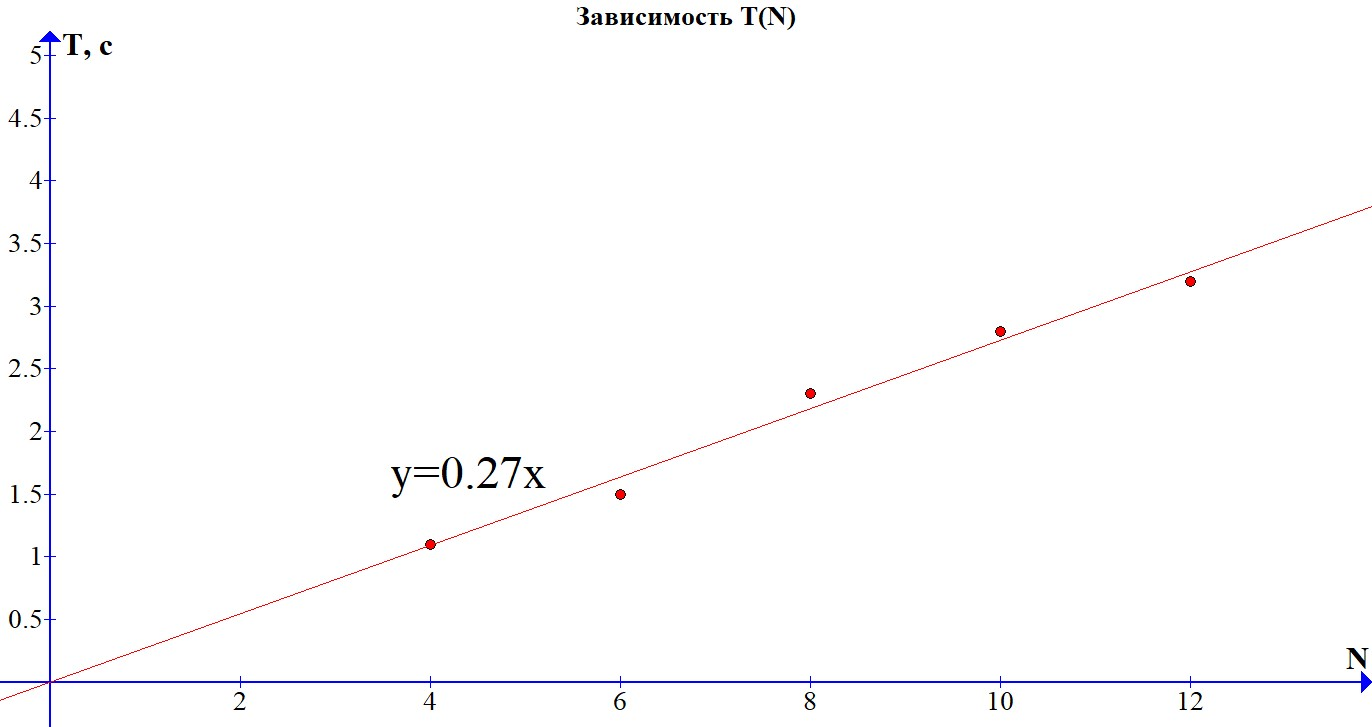
\includegraphics[scale=0.35]{1221}
\\
$Отсюда k=0.27, найдем горизонтальную составляющую поля Земли B_h=\frac{\pi^2 m d^2}{3k^2P_m}$=0.2 Гс
\\
\textbf{ Задание 3}\\
10) Изготовим магнитную стрелку из 10 шариков и повесим ее на штативе

11) Уравновесим стрелку с помощью кусочков медной проволоки. Рассчитав ее массу, снимем зависимость момента от количества шариков в стрелке. Результаты занесем в таблицу: \\
\begin{center}

\begin{tabular}{|c|c|c|c|}

\hline 
N & m, g & r, shar & M, $g*cm^4/c^2$ \\ 
\hline 
10 & 0.224 & 3 & 395.5 \\ 
\hline 
8 & 0.211 & 3 & 372.6 \\ 
\hline 
6 & 0.211 & 2 & 248.4 \\ 
\hline 
4 & 0.333 & 1 & 196 \\ 
\hline 
12 & 0.333 & 2 & 392 \\ 
\hline 
\end{tabular} 
\end{center}


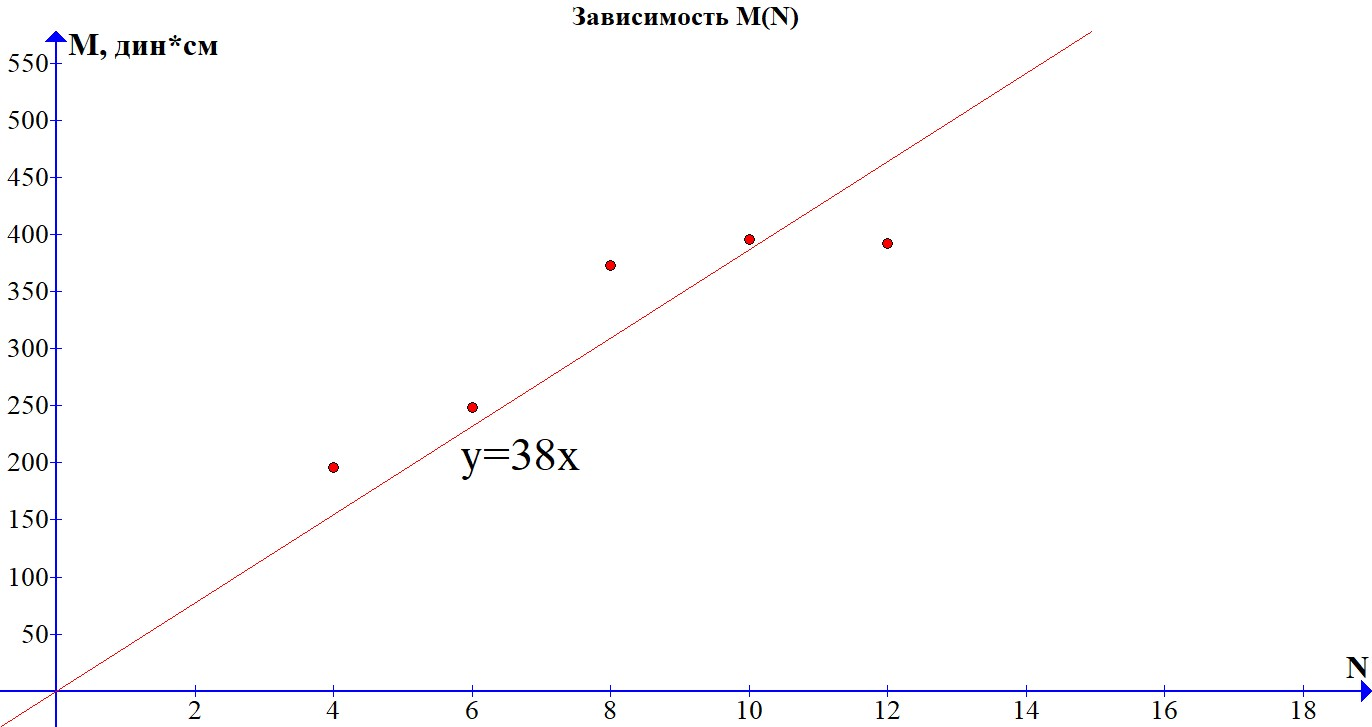
\includegraphics[scale=0.34]{1222}

12) Отсюда вертикальная составляющая поля Земли: \\ $B_v=\frac{K}{P_m}=0.54$Гс\\


Угол $\beta=57.3^{\circ}$, широта Долгопрудного - $56^{\circ}$































\end{document} % конец документа
